\documentclass[11pt, a4paper]{article}
\usepackage[utf8]{inputenc}
\usepackage[margin=1.2 in]{geometry}
\usepackage{graphicx}
\usepackage[T1]{fontenc}
\usepackage{charter}
\usepackage{amsmath}
\usepackage{setspace}
\usepackage{subcaption}
\usepackage{listings}
\usepackage{color}

\graphicspath{{Assets/}}

\title{CSCU9YE Assignment Report}
\author{Student no: 2519302}
\date{November 17\textsuperscript{th} 2018}
\pagenumbering{roman}
\begin{document}
\begin{titlepage}
\maketitle
\clearpage\thispagestyle{empty}
\end{titlepage}
\doublespacing
\setstretch{1}
\tableofcontents
\thispagestyle{empty}
\newpage
\singlespacing

\section{Introduction}

This project is tasked with the classification of spam emails, to a respectable degree of accuracy using machine learning models. Specifically, this project will employ a Support Vector Machine, Random Forest Classifier and Multilayer Perceptron Classifier. This report will aim to provide an overview of the datasets used, an understanding of how the models used work and the results obtained from running these models on the datasets mentioned.  

\section{Specification}

This section will walk through the flowchart shown in \emph{Figure~\ref{fig:flowchart}}.

\subsubsection*{Load Emails}

Firstly, the emails need to be loaded into the program in order to parse through them and begin the pre-processing stage. This involves reading in all the files in the folder and saving them to a variable for manipulation further on in the program. 

\subsubsection*{Pre-Process Data}

This stage is where the data is processed to convert case, remove elements such as punctuation and stop words and is where the process of lemmatization happens. This process is also referred to as normalization. These entities are removed due to their inherent lack of relevance to the end classification. Lemmatization on the other hand is done in order to reduce the complexity of the generated dictionary in the next step and thus  the overall runtime of the algorithms on the dataset.

\subsubsection*{Dictionary Creation}

This process, mentioned briefly above, entails the tallying of the most commonly occurring words in all the emails in the dataset. This is done such that a correlation can be obtained when reading through similar pieces of text. This allows us to see if the emails share similarities and thus may be classed under a label. The generated dictionary is then compared to the features extracted from each email.

\subsubsection*{Feature Extraction}

The feature extraction phase entails extracting a feature vector for all emails in the dataset. The features contain the number of occurrences of each entity in the email, with respect to the dictionary generated.  

\subsubsection*{Split Dataset}

The dataset is split into a test set and a training set. This is done such that the model can be trained on a subset of the dataset as a whole and the model can then be evaluated on the same data. The split is done at approximately 70 / 30, where the training set is 70\% of the full dataset and the remaining 30\% is used as the test set.

\subsubsection*{Train Model}

The models are trained with a subset of the dataset as mentioned above. 

\subsubsection*{Pre-Trained Model}

This process is where the pre-trained model is tested with the test set obtained from when the dataset was split.

\subsubsection*{Evaluate Trained Model}

The outputs of the models used here are evaluated using the performance matrices: Accuracy, Precision, Recall and F1-Score. The unlabelled dataset used here is the same test set, but without any accompanying labels designating the entities classification.

\subsection{Pseudocode}
Shown below is the pseudocode for the spam classification algorithm:
\begin{lstlisting}[frame=single]
begin spam_classification

    begin load_emails
        load emails into program
        split dataset into test set and training set
    end load_emails
	
    begin pre_processing
        convert text to lower case
        remove stop_words
        lemmatize text
    end pre_processing
	
    begin create_dictionary
        generate dictionary
    end create_dictionary
	
    begin feature_extraction
        extract feature vectors for all emails
    end feature_extraction
	
    Train models on training set
    Test models on test set
    Generate predictions using models
    Evaluate model predictions
    
end spam_classification
\end{lstlisting}
\newpage
\begin{figure}[h!]
\centering
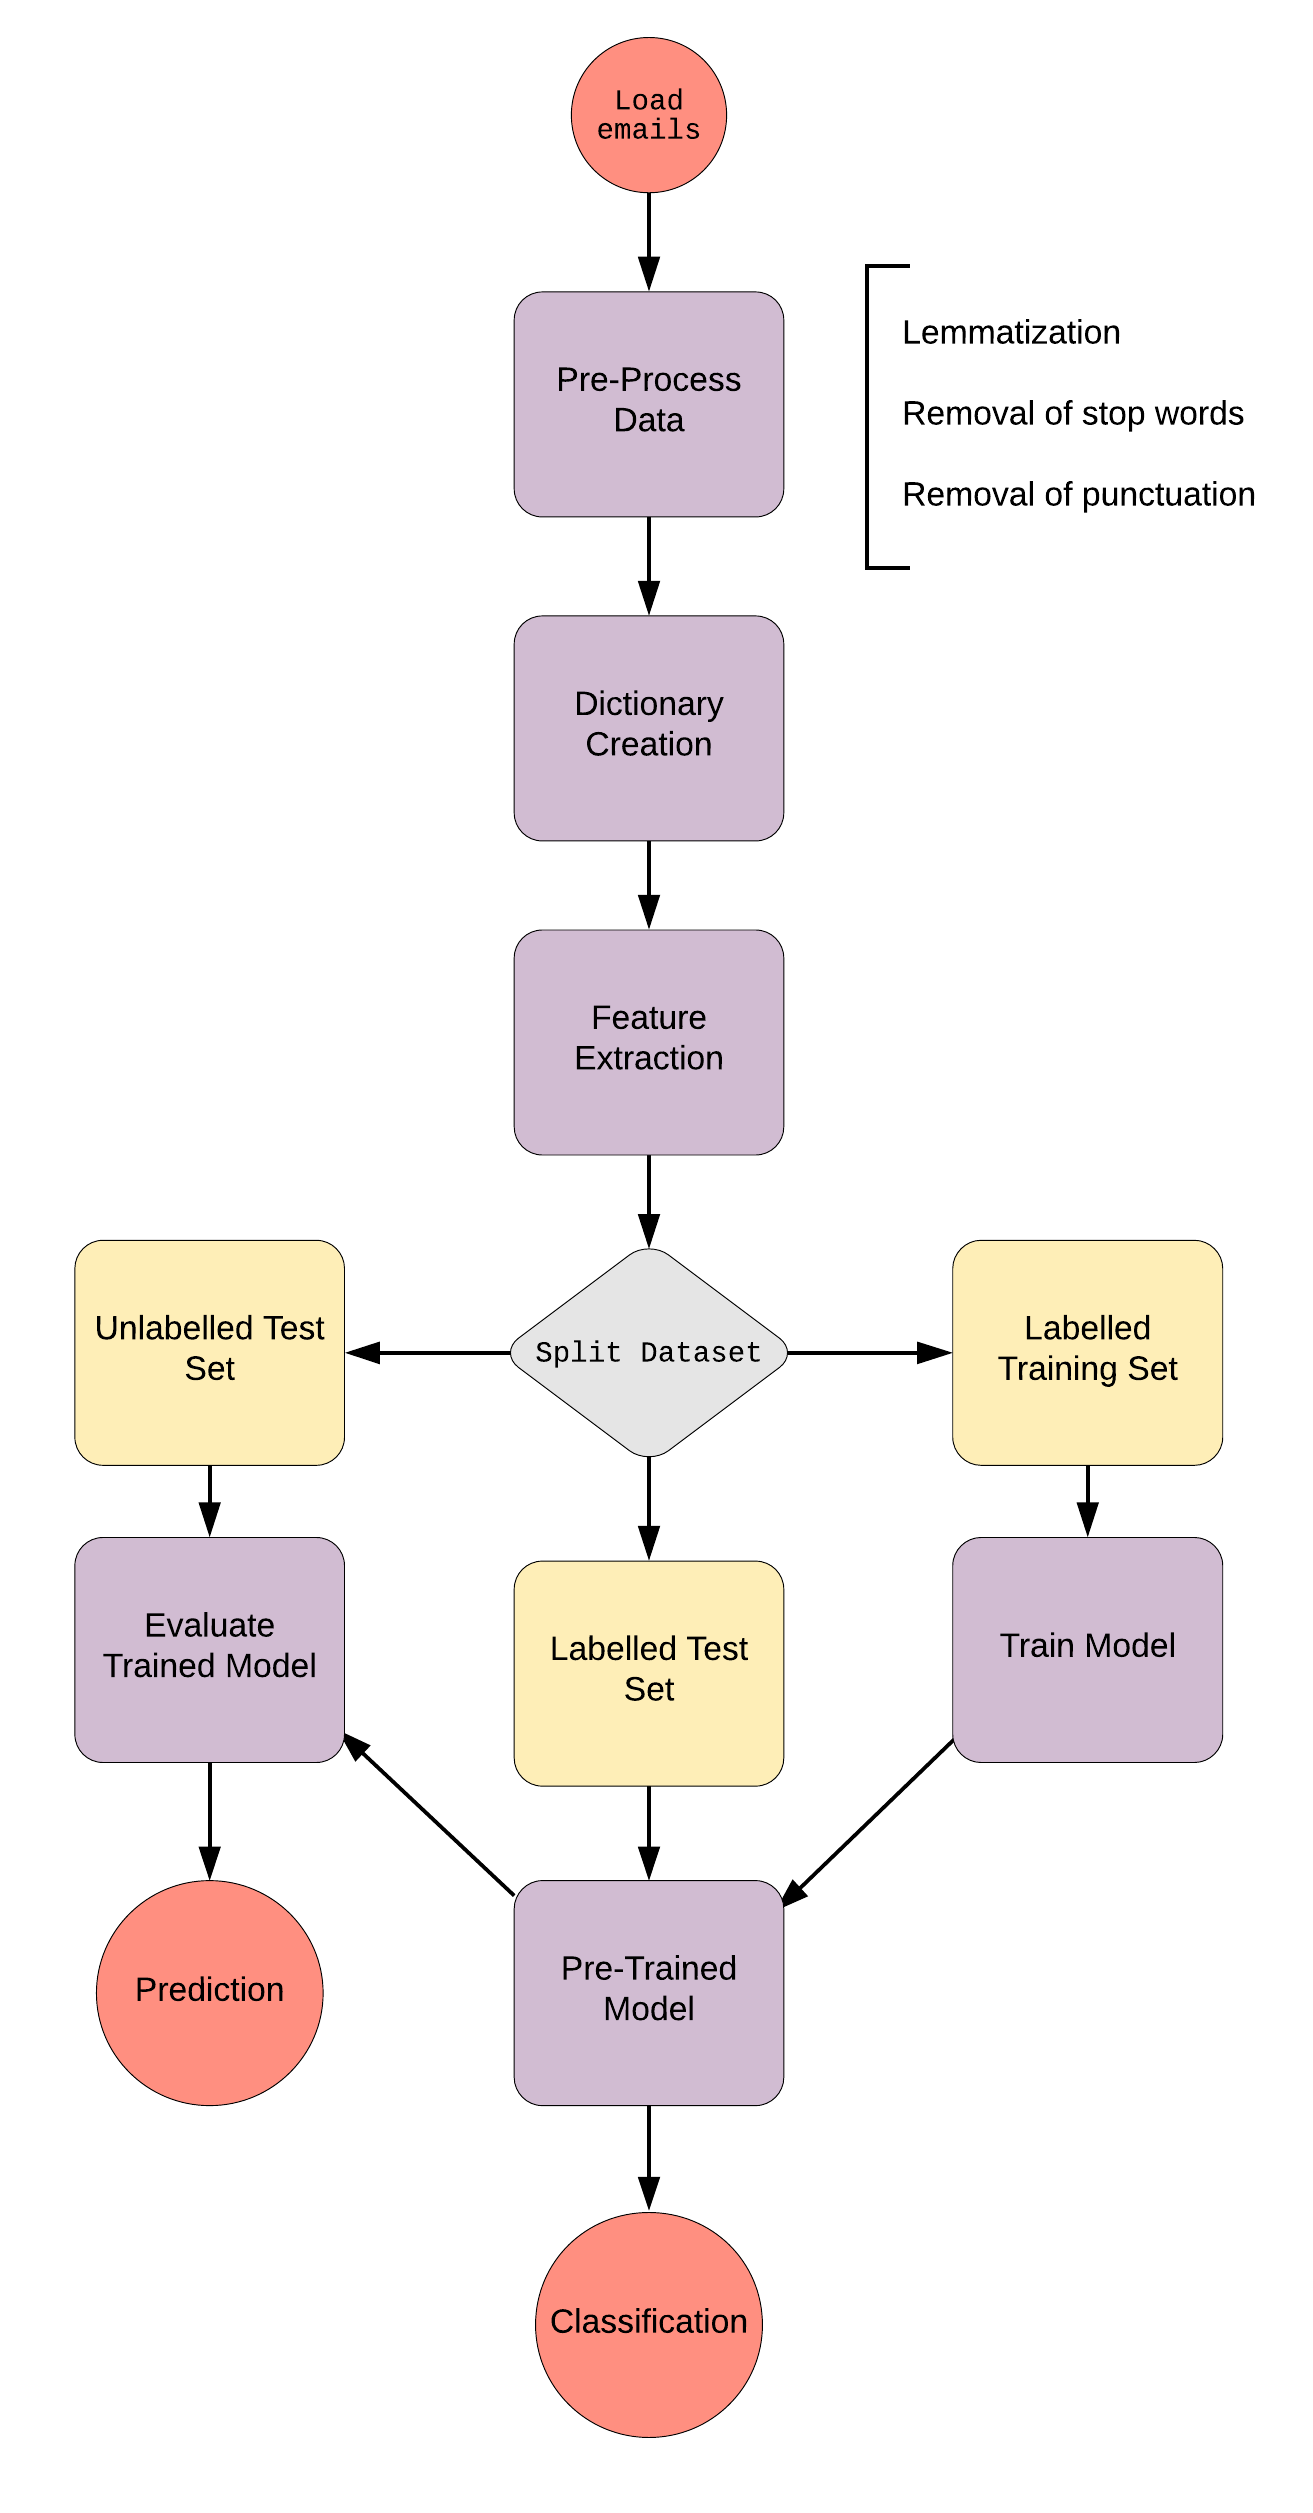
\includegraphics[scale=0.2]{spam_flowchart}
\caption{Flowchart for the general Spam Classification process}
\label{fig:flowchart}
\end{figure}
\newpage

\section{Pre-Processing}

This section will aim to cover the different aspects of pre-processing employed in this project. Within the datasets used in this project, we can see that the general steps one would need to take are as follows:
\begin{itemize}
\item Lemmatization
\item Removal of stop words
\item Removal punctuation
\end{itemize} 
Along with the aforementioned steps, the text will be processed to handle case. This is done by converting the text to lower case before any text normalization is done. 

\subsection{Lemmatization}

Lemmatization is a form of text normalization where the aim is to remove inflection and/or derive the base word from a family of words in the dataset \cite{schutze2008introduction,jabeen2018stem,fortney2017nlp}. The base of a word, is also known as the \textbf{lemma} or the \textbf{dictionary form}. This process also leads to a decrease in complexity during the runtime of the algorithm. An example of which is shown in \emph{Table \ref{table: lemma}} below.\\\\
Such mapping also allows us to find all relevant documents using a specific word.
\begin{table}[h!]
\centering
\begin{tabular}{c c c}
\hline
\textbf{Word} & & \textbf{Lemma}\\
\hline
\text{Cleaning} & \(\rightarrow\) & \text{Clean}\\
\hline
\text{Cleaner}  & \(\rightarrow\) & \text{Clean}\\
\hline
\text{Cleanliness} & \(\rightarrow\) & \text{Clean}\\
\hline
\end{tabular}
\caption{Showing the mapping of words to its lemma}
\label{table: lemma}
\end{table}

\subsection{Removal of Stop Words}

Stop words are words such as "the", "he" or "in". These words do not contribute to the overall meaning of the text and are thus removed during the pre-processing stage. This also tends to be done in order to improve indexing times for larger datasets.

\subsection{Removal of Punctuation}

Punctuation, like stop words are removed due to their lack of contribution to the overall understanding of the text.  

\newpage
\section{Machine Learning Methods}

This section will aim to provide some knowledge on the machine learning models employed in this project. 

\subsection{Support Vector Machine}

A Support Vector Machine (SVM) is a discriminative classification method. This method produces a classification by finding an optimal hyperplane that segregates the data points and thus returns classifications \cite{svm}. This can be visualized easiest on a 2-Dimensional plot as can be seen below in \emph{Figure \ref{fig:svm}}:
\begin{figure}[h!]
\centering
\begin{minipage}[]{0.45\textwidth}
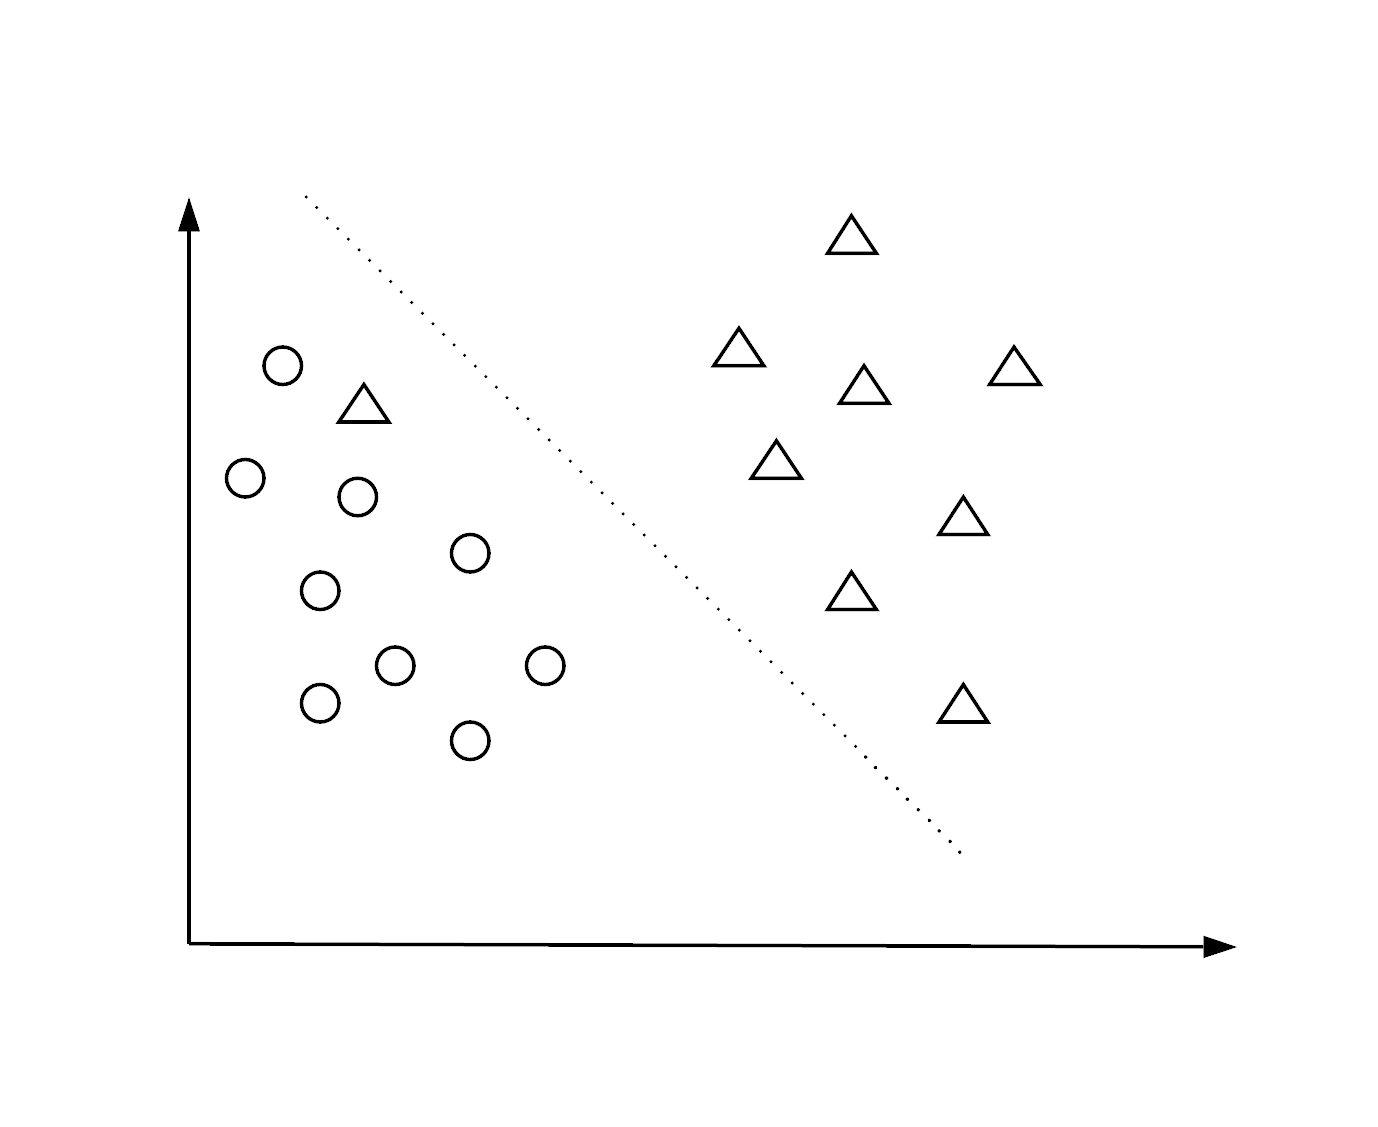
\includegraphics[scale=0.16]{svm}
\caption{SVM on 2-D plot area}
\label{fig:svm}
\end{minipage}
\hspace{0.5 cm}
\begin{minipage}[]{0.45\textwidth}
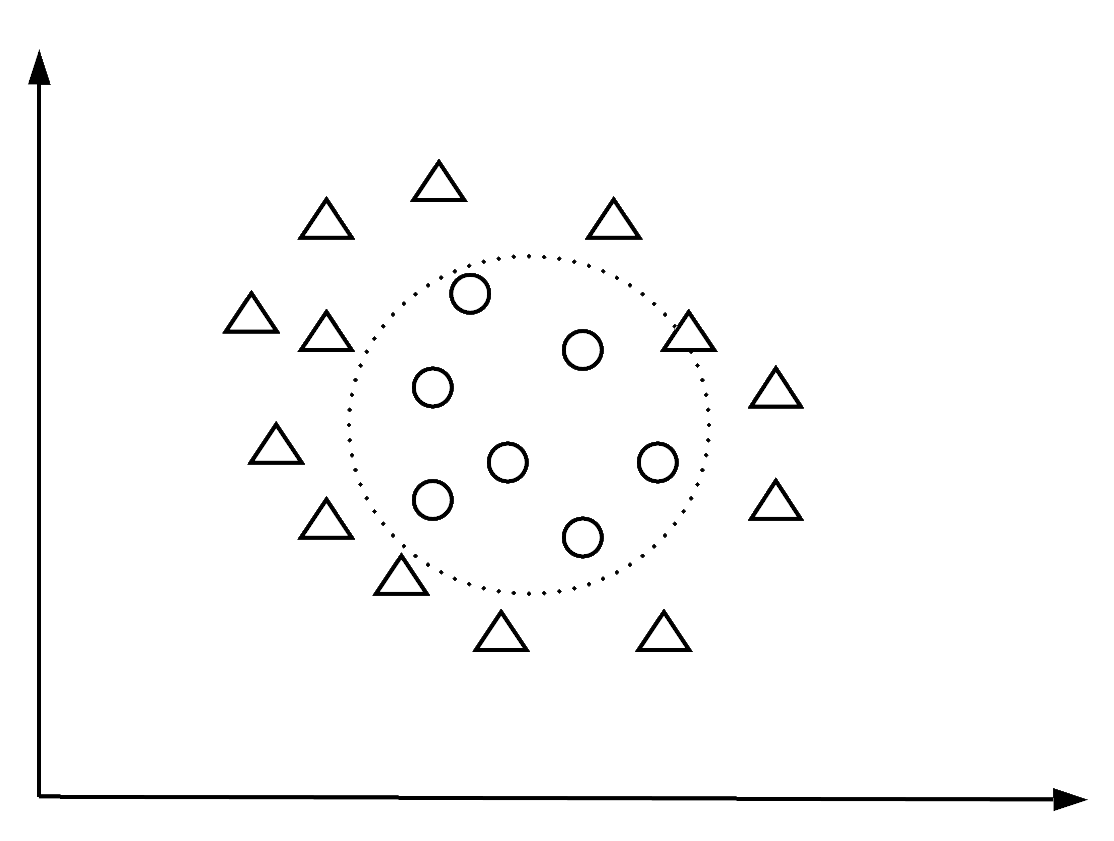
\includegraphics[scale=0.16]{svm_kernel}
\caption{Kernel feature of SVM}
\label{fig:svm_kernel}
\end{minipage}
\end{figure}

\emph{Figure \ref{fig:svm_kernel}} above shows an SVM making a classification on data where it would seem like there is no \emph{linear} hyperplane to be found. In order to make a classification, the SVM employs the kernel method \cite{ray2017svm}. This transformation, introduces a new dimension, by way of suggesting that for every \textbf{x} and \textbf{x'}, there is a function \emph{k} such that \emph{k} is equivalent to the sum of the squares of \textbf{x} and \textbf{x'} \cite{hofmann2008kernel}. This transformation then allows the model to find an optimal hyperplane within this third dimension. Transforming this back into a 2-Dimensional plot, the hyperplane is mapped as a circular boundary around the classified data points.

\subsection{Random Forest}

Random Forest is a supervised learning algorithm. The way it works is by generating a number of decision trees, all of which generate a classification. This is analogous to each decision tree in the forest 'voting' on a classification. The algorithm obtains a final singular classification by choosing the classification with the most 'votes'. To note, the decision trees generated by this algorithm are not pruned. 

\subsection{Multilayer Perceptron}

A Multilayer Perceptron (MLP), is a form of feedforward artificial neural network. Its general structure consists of an input layer, a number of hidden layers and an output layer. Within each of these layers there are neurons which compute an output based on an activation function. This activation function is different based on what sort of problem the MLP is being applied onto. In the case of this project, the activation function used is the ReLU, the rectified linear unit function.
 
Each neuron within each layer is connected by a weighted connection. This weight is randomly assigned at the start of the model's training epoch and is refined through the process of backpropagation. This process is how the MLP 'learns'. This process of backpropagation is repeated until the error from the output can no longer be reduced or is zero. At the end of this process, the model returns a classification. 
  
\section{Datasets Used} 

This section will provide a brief description of the datasets used in this project.

\subsection{Ling-Spam Dataset} 

The Ling-Spam dataset used in this project was that provided in the assignment brief. This dataset is a subset of the Ling-Spam corpus, a set of legitimate and spam emails sent via the Linguist list (a mailing list on linguistics). The original corpus consisted of 2893 emails, of which, 481 were spam and the remaining 2412 were legitimate. In the subset provided, the dataset consists of 962 total emails, both spam and legitimate. Of those emails, 702 were used in the training set and the remaining 260 were used as the test set. 

This dataset had already been neatly organized into a 50/50 split of spam and non spam emails in each respective subset, this allowed for a fairly simple process of pre-processing the data.

\subsection{Enron Dataset}

In addition to the dataset referred to above, this project will be using the Enron corpus of spam and legitimate emails. This corpus originally consists of 500,000 emails. The dataset used in this project however is a subset of that corpus, containing 33,699 emails. Of these emails, 17,154 were spam and 16,545 were legitimate. This dataset was split into a training set and test set using a ratio of 70 / 30 respectively.

An important thing to note is that this is not the subset in its entirety, since upon extraction of the files, the anti-virus software on my computer locked certain files from being able to be modified and thus needed to be removed from the dataset in order for the program to run.

\section{Measurement Metrics}

This section aims to provide an overview of the metrics used to evaluate the models run in this project. For the sake of brevity, the abbreviations used in the equations for each metric are listed below:
\begin{itemize}
\item \emph{TP} = True Positives 
\item \emph{FP} = False Positives 
\item \emph{TN} = True Negatives 
\item \emph{FN} = False Negatives.
\end{itemize}

\subsection{Accuracy}

Accuracy is a metric that evaluates the fraction of correct predictions a model has made with respect to the overall predictions the model has made~\cite{accuracy}. Formally, Accuracy for binary classification tasks is defined as such:\\
\begin{equation}
Accuracy = \frac{TP + TN}{TP + TN + FP + FN}
\end{equation}

\subsection{Precision}

Precision is a metric that calculates the proportion of correctly classified instances. A high precision value indicates a low amount of False Positives generated. This equation is formally defined as:\\
\begin{equation}
Precision = \frac{TP}{TP + FP}
\end{equation}

\subsection{Recall}

Recall is used to find the proportion of actual positive classifications are accurate. A Recall value of 1 indicates that the model provided no False Negatives.  This equation is formally defined as such:\\
\begin{equation}
Recall = \frac{TP}{TP + FN}
\end{equation}

\subsection{F1-Score}
The F1-Score provides the balance between the Precision and Recall values from the model outputs. In essence, the closer the F1-Score is to 1, the more accurate the model is in its classifications. This equation is defined as such:\\
\begin{equation}
F1-Score = 2 \left(\frac{Precision * Recall}{Precision + Recall}\right)
\end{equation}

\section{Results and Discussion}

This section will provide the results of the models running on the datasets as mentioned above in the report and aim to draw a conclusion from it. To note, for both datasets, the models were run with the same hyperparameters where applicable. This was done such that the produced results were affected solely by the dataset they were run on and not by any additional tuning for optimization within a specific search space. 

For the Support Vector Machine, the specific variation used from the \emph{scikit-learn} library was the \emph{LinearSVC}. It was run with a \emph{max\textunderscore iters} parameter of 5000. 

For the Random Forest Classifier, the model was run with a \emph{n\textunderscore estimators} parameter value of 2000. This means that it will generate 2000 Decision Trees in its Forest.
\newpage
The Multilayer Perceptron used was \emph{MLPClassifer} from the library and it was run with the following parameters:\\
\begin{itemize}
\item \emph{hidden\textunderscore layer\textunderscore sizes} = (6,6,6,6,6,6,6,5,5,5,5,5,2)
\item \emph{solver} = lbfgs
\item \emph{alpha} = 1e-05
\item \emph{random\textunderscore state} = 2
\end{itemize}

These parameters were chosen for the \emph{MLPClassifier} through a combination of reading through the \emph{scikit-learn} API for this specific model and looking at how each parameter affects the output of the model by testing different outputs on both datasets with different parameter settings. Additionally, looking through the conventions within this library for parameter settings depending on the size of the dataset greatly assisted in the final parameter settings used. 

\subsection{Results on Ling-Spam data}

The results obtained by running all the aforementioned models on the Ling-Spam dataset is as shown below:\\
\begin{table}[!h]
\centering
\begin{tabular}{c c c c c}
 & Accuracy & Precision & Recall & F1-Score\\
\hline
Linear SVM & 0.94615 & 0.93939 & 0.95385 & 0.94656\\
\hline 
Random Forest Classifier & 0.97308 & 0.95555 & 0.99230 & 0.97358\\
\hline
MLP & 0.98077 & 0.98449 & 0.97692 & 0.98069\\
\hline
\end{tabular}
\caption{Table showing results for machine learning models on Ling-Spam dataset}
\label{table:lingspam}
\end{table}

We can observe from the data as shown in \emph{Table~\ref{table:lingspam}} above, the Random Forest Classifier and MLP performed the best in the test set. It is interesting to note however that, although the MLP objectively performed better across the board compared to the Random Forest Classifier, it has a noticeably worse Recall score. This difference is not so significant that it adversely affects the classifications obtained, however it is noteworthy that Random Forest is known to perform well on binary classification problems.

\newpage

\subsection{Results on Enron data}

The results as obtained from running the models on the Enron dataset is as follows:\\
\begin{table}[!h]
\centering
\begin{tabular}{c c c c c}
 & Accuracy & Precision & Recall & F1-Score\\
\hline
Linear SVM & 0.96747 & 0.97112 & 0.96573 & 0.96842\\
\hline 
Random Forest Classifier & 0.97745 & 0.97418 & 0.98238 & 0.97826\\
\hline
MLP & 0.97063 & 0.97548 & 0.96745 & 0.97145\\
\hline
\end{tabular}
\caption{Table showing results for machine learning models on Enron dataset}
\label{table:enron}
\end{table}

We can immediately see from the data shown in \emph{Table~\ref{table:enron}} that there are a number of similarities observable from the results on the previous dataset. The Linear SVM is the poorest performing model, the MLP performing the best overall and the Random Forest Classifier performing almost similarly to the MLP, only performing better on Recall score. This does cement the idea that Random Forest does perform optimally for  

\newpage
\bibliography{references}
\bibliographystyle{ieeetr}
\newpage

\appendix

\definecolor{my_magenta}{rgb}{0.8, 0.2, 0.4}
\definecolor{my_blue}{rgb}{0.33, 0.56, 0.93}
\definecolor{my_gray}{rgb}{0.5,0.5,0.5}
\lstset{ %
  backgroundcolor=\color{white},   % choose the background color
  basicstyle=\small\ttfamily,        % size of fonts used for the code
  breaklines=true,                 % automatic line breaking only at whitespace
  captionpos=b,                    % sets the caption-position to bottom
  commentstyle=\color{my_gray},    % comment style
  escapeinside={\%*}{*)},          % if you want to add LaTeX within your code
  keywordstyle=\color{my_magenta},       % keyword style
  stringstyle=\color{my_blue},     % string literal style
  showspaces=false,
  showtabs=false,
  showstringspaces=false, 
}

\section{Code}

\subsection{utility.py}
\lstinputlisting[language=Python]{utility.py}
\newpage
\subsection{spam\textunderscore classifier.py}
\lstinputlisting[language=Python]{spam_classifier.py}

\end{document}
